\documentclass[11pt,leqno]{article}

\newcommand{\pathtotrunk}{./}
%auto-ignore
%!TEX root = pnas.tex

\def\bc{{\mathcal B}}
\def\btc{{\mathcal{BT}}}

\newcommand{\HC}{\operatorname{Hoch}}
\newcommand{\HH}{\operatorname{HH}}

\newcommand{\CM}[2]{C_*(\Maps(#1 \to #2))}
\newcommand{\CD}[1]{C_*(\Diff(#1))}
\newcommand{\CH}[1]{CH_*(#1)}

\newcommand{\cl}[1]{\underrightarrow{#1}}

\newcommand{\Set}{\text{\textbf{Set}}}
\newcommand{\Vect}{\text{\textbf{Vect}}}
\newcommand{\Kom}{\text{\textbf{Kom}}}
\newcommand{\Cat}{\mathcal{C}}

\newcommand{\cell}{\mathfrak{D}}

\newcommand{\into}{\hookrightarrow}
\newcommand{\onto}{\twoheadrightarrow}
\newcommand{\iso}{\cong}
\newcommand{\quism}{\underset{\text{q.i.}}{\simeq}}
\newcommand{\htpy}{\simeq}
\newcommand{\actsOn}{\circlearrowright}
\newcommand{\xto}[1]{\xrightarrow{#1}}
\newcommand{\isoto}{\xto{\iso}}
\newcommand{\quismto}{\xrightarrow[\text{q.i.}]{\iso}}
\newcommand{\diffeoto}{\xrightarrow[\text{diffeo}]{\iso}}
\newcommand{\htpyto}{\xrightarrow[\text{htpy}]{\htpy}}

\newcommand{\directSum}{\oplus}
\newcommand{\DirectSum}{\bigoplus}
\newcommand{\tensor}{\otimes}
\newcommand{\Tensor}{\bigotimes}

\newcommand{\selfarrow}{\ensuremath{\smash{\tikz[baseline]{\clip (0,0.36) rectangle (0.48,-0.16); \draw[->] (0,0.2) .. controls (0.6,0.8) and (0.6,-0.6) .. (0,0);}}}}

\newcommand{\bdy}{\partial}
\newcommand{\compose}{\circ}
\newcommand{\eset}{\emptyset}

\newcommand{\id}{\boldsymbol{1}}

\newtheorem{property}{Property}
\newtheorem{prop}{Proposition}
\newtheorem{thm}[prop]{Theorem}

\newenvironment{rem}{\noindent\textsl{Remark.}}{}

% \mathrlap -- a horizontal \smash--------------------------------
% For comparison, the existing overlap macros:
% \def\llap#1{\hbox to 0pt{\hss#1}}
% \def\rlap#1{\hbox to 0pt{#1\hss}}
\def\clap#1{\hbox to 0pt{\hss#1\hss}}
\def\mathllap{\mathpalette\mathllapinternal}
\def\mathrlap{\mathpalette\mathrlapinternal}
\def\mathclap{\mathpalette\mathclapinternal}
\def\mathllapinternal#1#2{%
\llap{$\mathsurround=0pt#1{#2}$}}
\def\mathrlapinternal#1#2{%
\rlap{$\mathsurround=0pt#1{#2}$}}
\def\mathclapinternal#1#2{%
\clap{$\mathsurround=0pt#1{#2}$}}

% references

\newcommand{\arxiv}[1]{\href{http://arxiv.org/abs/#1}{\tt arXiv:\nolinkurl{#1}}}
\newcommand{\doi}[1]{\href{http://dx.doi.org/#1}{{\tt DOI:#1}}}
\newcommand{\euclid}[1]{\href{http://projecteuclid.org/euclid.cmp/#1}{{\tt at Project Euclid: #1}}}
\newcommand{\mathscinet}[1]{\href{http://www.ams.org/mathscinet-getitem?mr=#1}{\tt #1}}
\newcommand{\googlebooks}[1]{(preview at \href{http://books.google.com/books?id=#1}{google books})}



% packages

\usepackage{tikz}
\usetikzlibrary{shapes}
\usetikzlibrary{backgrounds}
\usetikzlibrary{decorations,decorations.pathreplacing}
\usetikzlibrary{fit,calc,through}

\usepackage[all,color]{xy}
\SelectTips{cm}{}

\usepackage[pdftex,plainpages=false,hypertexnames=false,pdfpagelabels]{hyperref}

\usepackage{xcolor}
\definecolor{dark-red}{rgb}{0.7,0.25,0.25}
\definecolor{dark-blue}{rgb}{0.15,0.15,0.55}
\definecolor{medium-blue}{rgb}{0,0,0.65}

\hypersetup{
    colorlinks, linkcolor={dark-red},
    citecolor={dark-blue}, urlcolor={medium-blue}
}


%auto-ignore
%this ensures the arxiv doesn't try to start TeXing here.

%!TEX root = ../blob1.tex

\input{\pathtotrunk preamble.tex}

\newtheorem{lemma}[prop]{Lemma}

\usepackage[pdftex,plainpages=false,hypertexnames=false,pdfpagelabels]{hyperref}

\usepackage{breakurl}

\usepackage[pdftex]{graphicx}

%must load tikz after graphicx
\usepackage{tikz}
\usetikzlibrary{shapes}
\usetikzlibrary{backgrounds}
\usetikzlibrary{decorations,decorations.pathreplacing}
\usetikzlibrary{fit,calc,through}

\newtheorem{example}[prop]{Example}

\usepackage{color}

% This switches fonts to the Palatino family.
%\renewcommand{\familydefault}{ppl}

%%% futzing with margins following Dror (from Karoubi)
%\marginparwidth 0pt%
%\marginparsep 0pt

%\textwidth   5.5in%
%\textheight  9.0in%
%\oddsidemargin 12pt%
%\evensidemargin 12pt%

%\topmargin -.6in%
%\headsep .5in


% margin stuff
\setlength{\textwidth}{6.5in}
\setlength{\oddsidemargin}{0in}
\setlength{\evensidemargin}{0in}
\setlength{\textheight}{8.5in}
\setlength{\topmargin}{-.25in}

%!TEX root = ../blob1.tex

%%%%% excerpts from KW's include file of standard macros

\def\z{\mathbb{Z}}
\def\r{\mathbb{R}}
\def\c{\mathbb{C}}
\def\t{\mathbb{T}}

\def\du{\sqcup}
\def\bd{\partial}
\def\sub{\subset}
\def\subeq{\subseteq}
\def\sup{\supset}
%\def\setmin{\smallsetminus}
\def\setmin{\setminus}
\def\ep{\epsilon}
\def\sgl{_\mathrm{gl}}
\def\op{^\mathrm{op}}
\def\deq{\stackrel{\mathrm{def}}{=}}
\def\pd#1#2{\frac{\partial #1}{\partial #2}}
\def\lf{\overline{\cC}}
\def\ot{\otimes}

\def\nn#1{{{\it \small [#1]}}}
\long\def\noop#1{}

% equations
\newcommand{\eq}[1]{\begin{displaymath}#1\end{displaymath}}
\newcommand{\eqar}[1]{\begin{eqnarray*}#1\end{eqnarray*}}
\newcommand{\eqspl}[1]{\begin{displaymath}\begin{split}#1\end{split}\end{displaymath}}

% tricky way to iterate macros over a list
\def\semicolon{;}
\def\applytolist#1{
    \expandafter\def\csname multi#1\endcsname##1{
        \def\multiack{##1}\ifx\multiack\semicolon
            \def\next{\relax}
        \else
            \csname #1\endcsname{##1}
            \def\next{\csname multi#1\endcsname}
        \fi
        \next}
    \csname multi#1\endcsname}

% \def\cA{{\cal A}} for A..Z
\def\calc#1{\expandafter\def\csname c#1\endcsname{{\mathcal #1}}}
\applytolist{calc}QWERTYUIOPLKJHGFDSAZXCVBNM;

% \DeclareMathOperator{\pr}{pr} etc.
\def\declaremathop#1{\expandafter\DeclareMathOperator\csname #1\endcsname{#1}}
\applytolist{declaremathop}{pr}{im}{gl}{ev}{coinv}{tr}{rot}{Eq}{obj}{mor}{ob}{Rep}{Tet}{cat}{Maps}{Diff}{Homeo}{sign}{supp}{Nbd};



%%%%%% end excerpt




%\title{Blob Homology}
\title{Sandbox}
\begin{document}

\begin{align*}
\begin{tikzpicture}[baseline]
\node[draw] (c) at (0,0) [circle through = {(1,0)}] {$f$};
\node (d) at (c.east) [circle through = {(0.25,0)}] {};
\foreach \n in {1,2} {
	\node (p\n) at (intersection \n of c and d) {};
	\fill (p\n) circle (2pt);
}
\begin{scope}[decoration={brace,amplitude=10,aspect=0.5}]
	\draw[decorate] (p2.east) -- node[right=2ex] {$a$} (p1.east);
\end{scope}
\end{tikzpicture} & = 
\begin{tikzpicture}[baseline]
\node[draw] (c) at (0,0) [circle through = {(1,0)}] {};
\begin{scope}
\path[clip] (c) circle (1);
\node[draw,dashed] (d) at (c.east) [circle through = {(0.25,0)}] {};
\foreach \n in {1,2} {
	\node (p\n) at (intersection \n of c and d) {};
}
\node[left] at (c) {$f$};
\path[clip] (d) circle (0.75);
\foreach \y in {1,0.86,...,-1} {
	\draw[green!50!brown] (0,\y)--(1,\y);
}
\end{scope}
\draw[->,blue] (1.5,-1) node[below] {$a \times I$} -- (0.75,0);
\end{tikzpicture} \\
\begin{tikzpicture}[baseline]
\node[draw] (c) at (0,0) [ellipse, minimum height=2cm,minimum width=2.5cm] {};
\draw[dashed] (c.north) -- (c.south);
\node[right=6] at (c) {$g$};
\node[left=6] at (c) {$f$};
\end{tikzpicture} & =
\begin{tikzpicture}[baseline]
\node[draw] (c) at (0,0) [ellipse, minimum height=2cm,minimum width=2.5cm] {};
\node[right=9] at (c) {$g$};
\node[left=9] at (c) {$f$};
\draw[dashed] (c.north) to[out=-115,in=115] (c.south) to[out=65,in=-65] (c.north);
\begin{scope}
\path[clip] (c.north) to[out=-115,in=115] (c.south) to[out=65,in=-65] (c.north);
\foreach \y in {1,0.86,...,-1} {
	\draw[green!50!brown] (-1,\y)--(1,\y);
}
\end{scope}
\draw[->,blue] (.75,-1.25) node[below] {$a \times I$} -- (0,-0.25);
\end{tikzpicture} \\
\begin{tikzpicture}[baseline]
\node[draw] (c) at (0,0) [ellipse, minimum height=2cm,minimum width=2.5cm] {};
\draw[dashed] (c.north) -- (c.south);
\node[right=18] at (c) {$g$};
\node[left=10] at (c) {$f$};
\fill (0,0.4) node (p1) {} circle (2pt);
\fill (0,-0.4) node (p2) {} circle (2pt);
\begin{scope}[decoration={brace,amplitude=5,aspect=0.5}]
	\draw[decorate] (p1.east) -- node[right=0.5ex] {\scriptsize $a$} (p2.east);
\end{scope}
\end{tikzpicture} & =
\begin{tikzpicture}[baseline]
\node[draw] (c) at (0,0) [ellipse, minimum height=2cm,minimum width=2.5cm] {};
\node[draw,dashed] (d) at (0,0) [circle, minimum height=1cm,minimum width=1cm] {};
\draw[dashed] (c.north) -- (d.north) (d.south) -- (c.south);
\node[right=18] at (c) {$g$};
\node[left=18] at (c) {$f$};
\clip (0,0) circle (0.5cm);
\foreach \y in {1,0.86,...,-1} {
	\draw[green!50!brown] (-1,\y)--(1,\y);
}
\end{tikzpicture} \\
\end{align*}

\begin{tikzpicture}
\node[circle,fill=black,inner sep=1pt] (A) at (1.73,0) {};
\node[circle,fill=black,inner sep=1pt] (B) at (-1.73,0) {};
\draw[dashed] (A) -- (B);
\node[circle,fill=black,inner sep=1pt] (C) at (0,0) {};
\node[circle,fill=black,inner sep=1pt] (D) at (0.8,0) {};
\begin{scope}[yshift=-1cm]
\path[clip] (0,0) circle (2);
\begin{scope}[yshift=2cm]
\draw (0,0) circle (2);
\node[circle,fill=black,inner sep=1pt] (L2) at (-90:2) {};
\node[circle,fill=black,inner sep=1pt] (L1) at (-120:2) {};
\end{scope}
\end{scope}
\begin{scope}[yshift=1cm]
\path[clip] (0,0) circle (2);
\begin{scope}[yshift=-2cm]
\draw (0,0) circle (2);
\node[circle,fill=black,inner sep=1pt] (U) at (90:2) {};
\end{scope}
\end{scope}
\begin{scope}
\path[clip] (0,1) circle (2);
\path[clip] (0,-1) circle (2);

\end{scope}
\end{tikzpicture}
\end{document}
